Visual information is vital for various robotic tasks deployed on mobile edge devices (mobile robots), such as navigation~\cite{ran2017convolutional}, manipulation~\cite{bayar2018constrained}, and human-robot interaction~\cite{wu2019weight};
and as a major visual information processing method, fast, accurate and energy-efficient visual model inference (typically convolution neural networks~\cite{kapao,targ2016resnet,woo2023convnext}) is important for the robotic tasks to timely respond to environment changes. 
Unfortunately, the mobile robot typically has limited computational power and limited and unstable wireless network bandwidth~\cite{yang2022mobile}, which slow down the inference speed via both local computation (complete all inference calculations on the edge device itself) and computation offloading (offload the calculations to remote GPU servers).
Thus the mobile robot often suffers the problem of slow visual model inference that interferes the robotic task performance (e.g., 1.xx seconds in human pose estimation~\cite{kapao} or 2.xx seconds in surrounding occlusion prediction~\cite{agrnav}) and the prolonged inference latency naturally increases energy consumption each inference.
% Unfortunately, the mobile robot typically has limited computational power and limited and unstable wireless network bandwidth~\cite{yang2022mobile}, which slow down both local computation on the mobile robot and naive offloading of computation to GPU servers.
% Thus the mobile robot often suffers slow visual model inference that interferes the robotic task performance (e.g., 1.xx seconds in human pose estimation~\cite{kapao} or 2.xx seconds in surrounding occlusion prediction~\cite{agrnav}).
% Unfortunately, the mobile robots often suffer slow visual model inference, due to their limited computational power and the limited and unstable wireless network bandwidth~\cite{yang2022mobile}, which slows down both local computation and naive offloading of computation to GPU servers.

To address this problem, we seek enlightenment from previous work targeting fixed-position edge devices (e.g., smart cameras) that employ caching mechanisms~\cite{cavigelli_cbinfer_2017,buckler_eva_2018,huynh_deepmon_2017} to reduce the computational burden of visual model inference.
They are based on the fact that the visual models extensively use operators (e.g., convolution) whose computation results (i.e. activations) are spatially correlated to the input image: the value of each pixel on the activations is dominated by a block of the input image (i.e., receptive field) determined by the model architecture~\cite{buckler_eva_2018}.
% Given a continuous stream of images, they either 1. recognize the movements of the receptive fields and interpolate (reuse) the cached activations of an operator accordingly to skip the activation computation of this and the previous operators, or 2. in cases of movements recognition failure, execute full local computation (recompute) on the input image to get the latest activations.
Given a continuous stream of images, these methods identify the movements of the receptive fields and interpolate (reuse) the cached activations of the corresponding operator, eliminating the need for computing activations for all related operators (including both the current and previous ones). 
When the movement recognition fails, a full local computation (recompute) is performed on the input image to obtain the latest activations by recomputing all the operators.

% While introducing such mechanism to reuse the cached previous activations to visual model inference on mobile robots seems able to skip local activation computation and reduce transmission data volume in computation offloading (since only recognized movements needs to be transmitted), it faces a \textbf{\textit{dilemma}} between inference accuracy and inference speed on mobile robots which feature frequent camera perspective movements~\cite{cavigelli_cbinfer_2017,huynh_deepmon_2017}.
Introducing a caching mechanism that reuses previous activations for visual model inference on mobile robots has the potential to eliminate activation computation and reduce data transmission volume in computation offloading (since only the receptive fields with recognized movements need to be recomputed and transmitted);
however, the frequent camera perspective movements~\cite{cavigelli_cbinfer_2017,huynh_deepmon_2017} inherent to mobile robots create a \textbf{\textit{dilemma}} between inference accuracy and inference speed when applying such caching mechanisms.
Changes in camera perspective typically bring new scenes or changed occlusion into the images, which cannot be covered by receptive field movements (recognition failure).
To cope with this situation, the above methods can only either ignore certain recognition failure at the cost of severely degraded inference accuracy (25.89\% lower in~\cite{huynh_deepmon_2017}), or frequently execute full local computation or full transmission of the input images during computation offloading, sacrificing inference speed.
Consequently, existing caching mechanisms struggle to strike a balance between inference accuracy and speed, regardless of whether they employ local computation or computation offloading.
% When camera perspective moves, possibly new scenes or changed occlusion cause the consecutive images to differ in a way that cannot be covered by receptive field movements, and such changes happen on a small portion (e.g., 5\%) of the pixels on the input image will cause a larger portion (e.g., 25\%) of pixels on the activations to change, because the receptive fields are often larger than a pixel (e.g., 20X20) and overlap.
% Simply introducing such caching mechanism seems able to accelerate both local computation and computation offloading by either skipping local activation computation or only necessitating the transmission of the recognized movements of receptive fields during computation offloading. But we 
% \begin{figure}
%     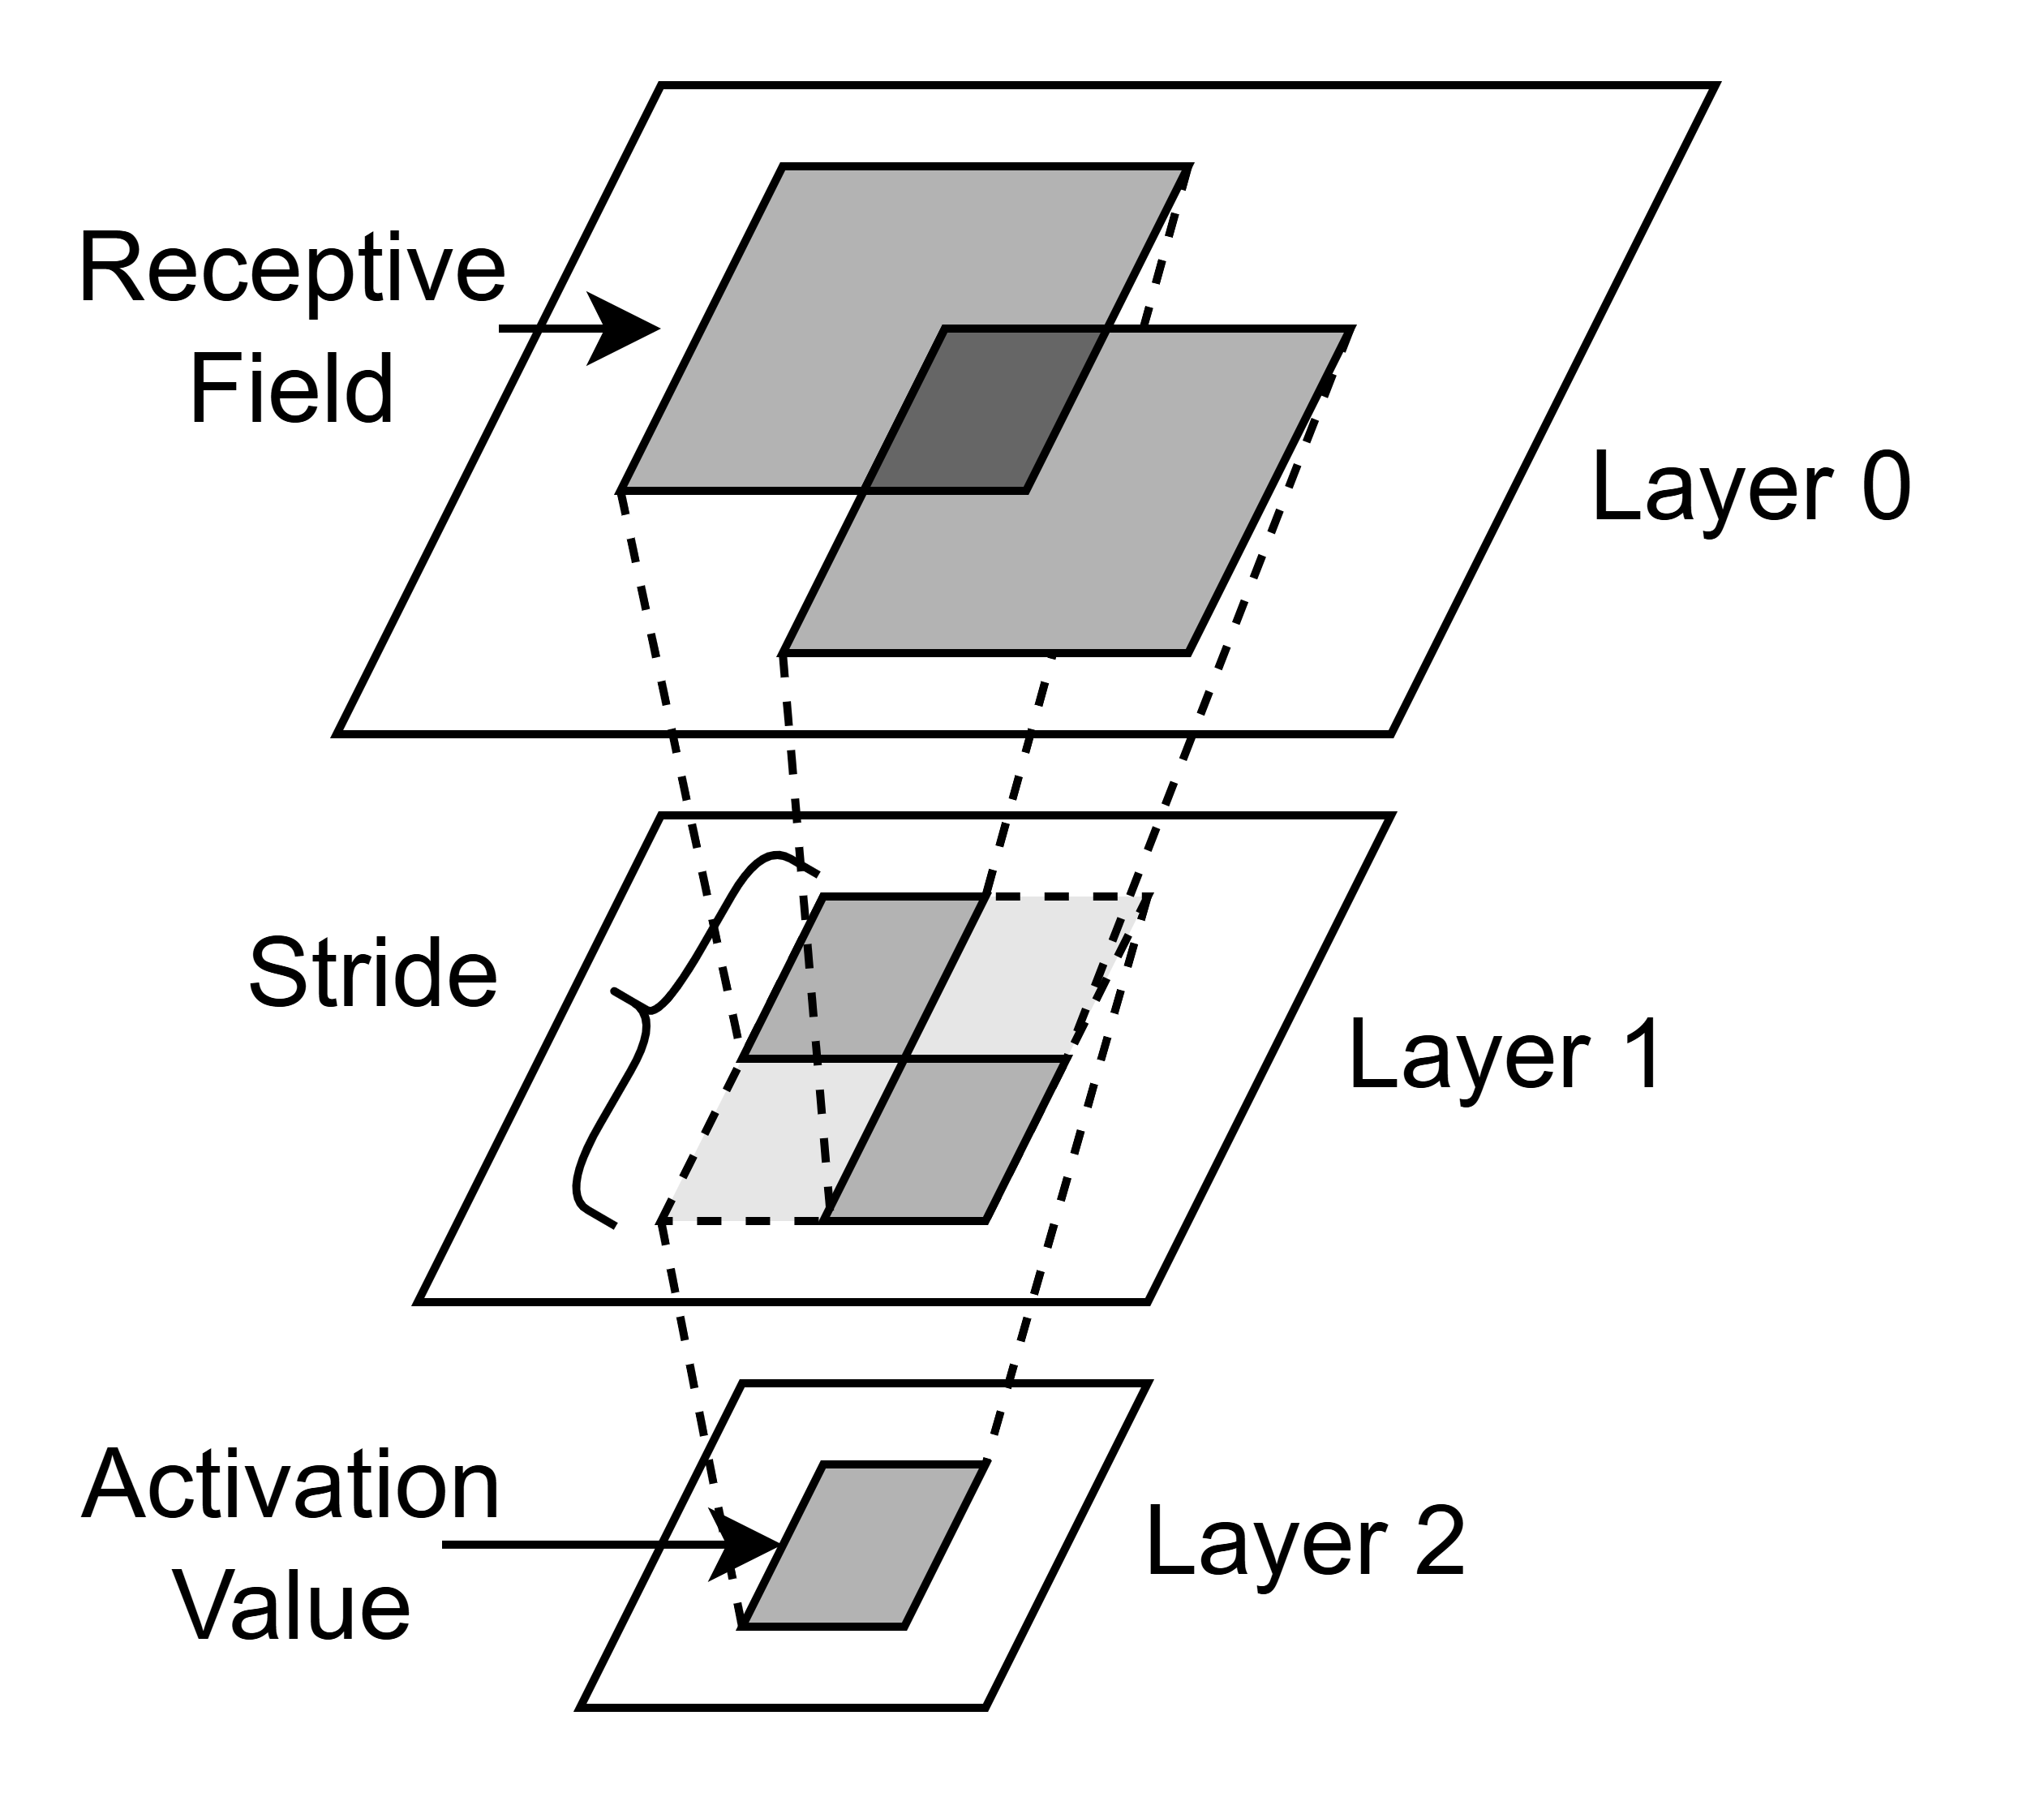
\includegraphics[width=0.5\linewidth]{fig/insight.drawio.png}
%     \caption[short]{Receptive fields and their dominated pixels on the activations.}
%     \label{fig:receptive field}
% \end{figure}

The key reason for the dilemma faced by existing caching methods is that they involve deciding whether to reuse or recompute the activations at the granularity of the whole input frame, which lacks a tradeoff space between inference accuracy and speed.
% The key reason to their dilemma is that while reusing or recomputing the activations optimizes the inference speed or accuracy and sacrifices the opposite, there lacks a tradeoff method between inference accuracy and speed.
% The key reason to their dilemma is that between wholly reusing or recomputing the activations which sacrifices accuracy or inference speed, there lacks an intermediate option that allows partial reusing and partial recomputing the activations to tradeoff between accuracy and inference speed.
When continuously reusing activations computed with a reference frame, the difference between the new frames and the reference frame accumulates, causing either degraded accuracy or triggering a full recomputation to eliminate errors in activations. 
However, with the ability to tradeoff between accuracy and inference speed (for example, partially reusing and partially recomputing the activations), we can selectively compute on the blocks with the most significant differences while reusing the computation results of the others, mitigating the accumulation of errors while accelerating both local computation and computation offloading via caching.
% When continuously reusing activations computed with a reference frame, the difference between the new frames and the reference frame accumulates and causes either degraded accuracy or triggering of full recomputation to eliminate error in activations; but with the ability to tradeoff between accuracy and inference speed (for example, partially reusing and partially recomputing the activations), we can selectively compute on the blocks with most differences while reusing the computation results of the others, mitigating the accumulation of error while accelerating both local computation and computation offloading via caching. 


% Given a continuous stream of images, they recognize the movements of the receptive fields (represented by motion vectors of the receptive fields) by matching similar pixel blocks on the consecutive input images and interpolate the activations accordingly to form the new activations, skipping the computation of the activations with the local operators and thus accelerating local computation.

% It is based on the facts that the input for the robotic visual models is typically a continual stream of images and these models mostly compute on the images using local operators (i.e., operators such as convolution that rely on local geometries of the input images)~\cite{o2015introduction,tripp2019approximating}.
% In such cases, computation results of similar local geometries between consecutive images can be reused to shrink the overall size of the computation, which reduces both local computation time and transmission time when offloading computation to the GPU server.

% Distributed inference has emerged as a promising approach to accelerate inference on robots by leveraging GPU servers (e.g., edge devices with powerful GPUs) via the Internet of Things for robots (robotic IoT). 
% While various parallel methods have been proposed and proven efficient in robotic IoT~\cite{sun2024hybridparallel}, the communication cost between the robot and GPU server remains a significant bottleneck, especially in robotic IoT environments with limited bandwidth.

% To address the challenge of high communication costs in distributed inference for robotic IoT, we propose leveraging the classic caching mechanism, which has proven efficient and widely used in robotic visual tasks. 
% By exploiting the fact that robotic visual models typically process a continual stream of images using local operators (e.g., convolution) that rely on local geometries of the input images~\cite{o2015introduction,tripp2019approximating}, the caching mechanism performs complete inference on key frames and reuses the cached results for the following consecutive frames, thus reducing their computational burden. 
% This approach effectively shrinks the overall size of the computation and reduces the required communication volume between the robot and GPU server. 
% Consequently, our proposed method accelerates the distributed inference of robotic visual models, demonstrating the potential of combining distributed inference and caching to achieve a synergistic effect greater than the sum of their individual benefits.

% To address the challenge of slow visual model inference on mobile robots, we propose leveraging the classic caching mechanism into robotic visual model inference has the potential to accelerate both local computation and offloading the computation to GPU servers.
% It is based on the facts that the input for the robotic visual models is typically a continual stream of images and these models mostly compute on the images using local operators (i.e., operators such as convolution that rely on local geometries of the input images)~\cite{o2015introduction,tripp2019approximating}.
% In such cases, computation results of similar local geometries between consecutive images can be reused to shrink the overall size of the computation, which reduces both local computation time and transmission time when offloading computation to the GPU server.

% However, simply combining distributed inference and caching mechanisms together faces significant challenges. 
% First, existing caching systems suffer from the dilemma between the accuracy of inference results and reduced computation burden, which is more costly in distributed inference on robotic IoT. 
% To reduce the cumulative error on the inference results caused by recomputation based on the same cache result, existing caching systems need to perform complete inference on the key frames frequently, which fails to effectively reduce the computational burden through caching. 
% Such complete inference incurs significant communication costs for distributed inference on robotic IoT and should be avoided as much as possible without compromising the accuracy of the inference results.

% Second, existing caching systems ignore the cost of reusing previous cache results. 
% These systems are designed for interactive generative image editing on high-end PCs, where the cache results are allocated on the PC, and the reusing cost can be ignored. 
% However, when applied to distributed inference, the cache results are allocated between the robot and the GPU server, and reusing costs (i.e., extra communication cost due to the limited and unstable wireless network bandwidth) should be considered. 
% Therefore, a new caching system specifically tailored for combining with distributed inference on robotic visual models is desired.

% However, existing caching systems for visual models, designed for interactive generative image edition on high-end PCs, are unfit for robotic tasks on mobile robots~\cite{li_efficient_2023}.
% With their targeted scenario, they assume no perspective changes in the images, consume excessive memory by caching computation results of every local operator and lack consideration for the acceleration opportunities provided by offloading computation to GPU servers.
% A new caching system specifically tailored for the unique requirements of robotic visual model inference is desired.

% However, there is a major gap to apply the existing caching systems for visual models to robotic tasks on mobile robots.
% They are designed for interactive generative image edition on high-end PCs which assumes no image perspective transformation, consumes too much memory and does not consider the acceleration opportunity of offloading, unfit for robotic tasks on mobile robots.

% When such gap is fulfilled and caching of computation results on consecutive images is enabled in robotic tasks on mobile robots, on one hand local computation time will be reduced by reusing cache, on the other hand we can collaboratively consider cache both on the robot and the offloading server and further reduce transmission data volume when offloading computation to the server.
% Enabling caching 
% Filling such gap would 


% To tackle this problem, we seek opportunity from the facts that the input for the robotic visual models are typically a continual stream of images and the models mostly compute on these images using local operators (i.e., operators such as convolution that relies on local geometries of the input images).
% These imply that between visual model inference on consecutive images in visual robotic tasks, part of the previous computed results of local operators can be cached and reused, providing opportunity to both reduce local computation time and reduce transmission data volume, accelerating the overall visual model inference.

To bridge this gap, in this paper, we propose CacheInf, a high-performance collaborative edge-cloud cache system for efficient robotic visual model.
% To bridge this gap, in this paper, we propose CacheInf, a collaborative edge-cloud cache system for efficient robotic visual model inference.
% Given a continuous stream of visual input in a robotic visual task, CacheInf analyses the overlapping area between consecutive inputs;
Given a continuous stream of visual input in a robotic visual task, CacheInf selectively reuses a portion of the cached activations of a reference frame while recomputes the rest based on statistical metrics such as the mean square error of pixels in corresponding receptive fields between the reference frame and the current frame.
In this way, the amount of required computation is minimized which accelerates both local computation and computation offloading and the error accumulation in activations is mitigated, achieving the optimal tradeoff between inference accuracy and inference speed for collaborative edge-cloud visual model inference on the mobile robot.

% The first challenge of the design of CacheInf is how to distinguish the parts of the input image to recompute and update the activations so that we can maintain high inference accuracy.
% When perspective changes along a video stream are involved, the appearance of the background, besides the targeted objects, will gradually change, disabling the traditional appearance based metrics such as mean square error between corresponding pixel blocks.
% We propose to use the variance 

The first challenge of the the design of CacheInf is to minimize computation using cache mechanism without compromising the inference accuracy.
While prioritizing recomputation on receptive fields with most appearance difference seems effective, the background also gradually changes in appearance along a video stream with perspective changes, which attracts wasteful recomputation on these areas.
We observe that a moving targeted object tend to have different movements compared with the background (otherwise it is stationary and the corresponding cached activations can be directly reused).
Thus, instead of appearance-based metrics, we analyze the movements of the sub-pixel blocks of a receptive field (internal movements) and prioritize the recomputation on receive fields with highest variance in internal movements, reducing unnecessary computation while maintaining high inference accuracy.

%  we also notice under the same level of difference between consecutive images, if we choose to cache the activations computed by an operator closer to the input image (former), the portion of activations needed to be recomputed would be reduced.
% This is because the former operators have smaller receptive fields compared with the latter ones whose activations are less affected by difference across images, but there are more operators after the cached operator whose computation are not skipped.

% Based on these observations, we design a mechanism in CacheInf to both selectively and adaptively choose the operator to cache its computed activations and the portion of activations to be recomputed according to the levels of difference across input images detected and the amount of possible computation reduction, achieving maximal computation reduction while maintaining high inference accuracy.

The second challenge is to minimize the overall inference latency considering the interaction between the mobile robot and the GPU server.
One major obstacle is that switching between local computation and computation offloading under the caching mechanism (e.g., when wireless network bandwidth changes) typically requires costly one full local recomputation or full transmission of the input image, and such cost hinders a greedy scheduling method from adopting such switching to gain further overall acceleration.
To overcome this issue, we schedule between local computation and computation offloading by looking ahead several steps with the predicted future wireless network bandwidth and possible computation reduction based on previous records, to minimize the overall inference latency.

We implement CacheInf based on python and pytorch integrated with self-implemented C++ cuda extensions.
For the tail cases where we need to fully offload an input image to the GPU server, we integrate a state-of-the-art offloading method called Hybrid-Parallel (HP)~\cite{sun2024hybridparallel} which mitigates the caused latency.
Our baselines include HP, a state-of-the-art cache-based computation reduction methods called EVA2~\cite{buckler_eva_2018}, EVA2 integrated with HP and local computation.
We evaluated CacheInf on a four-wheel robot equipped with a Jetson NX Xavier~\cite{jetsonnx} that is capable of computing locally with its low-power-consumption GPU.
The offloading GPU server is a PC equipped with an Nvidia 2080ti GPU.
Our datasets include the standard datasets of video frames of DAVIS~\cite{Perazzi2016} and CAD~\cite{Choi_VSWS_2009} each captured by a handheld camera and our self-captured video frames using sensors on our robot.
Extensive evaluation over various visual models~\cite{kapao,agrnav,noauthor_torchvision_nodate} and wireless network bandwidth circumstances shows that:
\begin{itemize}
    \item CacheInf is fast and accurate. Among the baselines, CacheInf reduced the end-to-end inference time by 13.1\% to 48.8\% with only 0.21\% to 0.96\% accuracy reduction.
    \item CacheInf saves energy. Among the baselines, CacheInf reduced the average energy consumed to complete inference on each image by 9.5\% to 39.9\%.
    \item CacheInf is robust. Under different level of difference across consecutive input images, the advantages of CacheInf remained.
\end{itemize}

The contribution of this paper is twofold: 1. a new caching mechanism for visual model inference on mobile devices which selectively reuse and recompute fractions of cached activations to best tradeoff between inference accuracy and computation reduction; 2. a scheduling mechanism designed to optimize the overall inference latency considering the interaction between the edge (the mobile robot) and the cloud (the GPU server to offload computation to)
And the resulting system, CacheInf, optimally reduces visual model inference latency and energy consumption on the mobile robot.
The accelerated visual model inference and the reduced power consumption will make real-world robots more performant on various robotic tasks and nurture more visual models to be deployed in real-world robots.
The source code and evaluation logs of CacheInf is available at \MYhref{todo}{todo}.

The rest of this paper is organized as follows.
Chapter two introduces background and related work.
Chapter three gives an overview of CacheInf and Chapter four presents its detailed design.
Chapter five describes the implementation.
Chapter six presents our evaluation results and Chapter seven concludes.




% Given a continuous stream of visual input in a robotic visual task, CacheInf recognizes the reusable portion of activations whose receptive field movements are recognized and for  while the rest portion are non-reusable portion of activations the overlapping area between consecutive inputs;
% based on the portion of overlapping area (reusable cache) and the current estimated wireless network bandwidth, CacheInf schedules the action between reusing local cache to reduce local computation time and reusing the remote cache (e.g., the cache at the GPU server side from the robot's perspective) to minimize transmission time when offloading, ultimately reducing the overall visual model inference latency.
% Schedule cache and offloading...
% Reduce data volume transmission in offloading at higher bandwidth...
% At low bandwidth where offloading is not feasible, reduce local computation time...

% The design of CacheInf is non-trivial.
% The first challenge is deciding which parts should reuse previous cache results, avoiding complete inference on key frames as much as possible without compromising the accuracy of inference results. 
% % The first challenge is to transform cached results to local computation acceleration.
% While the computation of cached areas can be skipped, the remaining uncached areas need computing but can not be computed on the highly optimized local operators for dense local geometries (e.g., conv2d in pytorch~\cite{paszke2017automatic}), since these areas are typically sparse and fragmented, hindering acceleration.
% (TODO) To address this problem, we designed and implemented sparse local operators based on the optimized sparse spatial data structure in taichi~\cite{taichi}, which achieved comparable performance with the default local operators for dense local geometries in pytorch~\cite{paszke2017automatic} and the computation results on sparse uncached areas can be simply combined with the cache to recover the corresponding global geometry.
% In this way, CacheInf transforms some key frames into consecutive frames with residual replenishment based on motion vectors, effectively maintaining the accuracy of inference results while minimizing the need for complete inference on key frames.

% The second challenge is properly scheduling the computation and reuse of different parts to achieve fast distributed inference. 
% (TODO) CacheInf addresses this challenge by introducing a novel scheduling strategy (XXX) that determines the corresponding distributed inference methods while considering the cost of reusing previous cache results. 
% XXX formulates the problem as a nonlinear optimization problem and schedules the computation and reuse of different parts based on the solution obtained via the differential evolution algorithm.


% % The second challenge is how to reduce the cache memory consumption, especially at the robot side which typically has a tight GPU memory budget.
% % In visual models, the computation results of local operators often consume significantly more memory than the parameters of the local operators themselves and naively caching all the computation results leads to a heavy GPU memory burden.

% We observe that in visual models, the computation result of a local operator often serves as the input of another local operator. 
% In this case, the computation result of the sparse uncached areas of a local operator can be passed to the following local operators without loss of information, allowing the cache between these two operators to be ignored or merged with the first operator to reduce memory consumption.
% We greedily search for opportunities to merge cache for each operator and balance between sparse computation acceleration and GPU memory consumption.
% % We greedily search for a continuous sequence of local operators whose starting and ending operators incur the least memory consumption and cache the computation results of the starting and ending operators only, so as to minimize cache memory consumption.

% To fully exploit the potential acceleration of cache and offloading, we integrate an emerging offloading paradigm named Hybrid-Parallel~\cite{sun2024hybridparallel}: during visual model inference on an image, Hybrid-Parallel enables splitting of the input of local operators and assigns different splits to the local robot and the remote GPU server for computation, allowing local computation and data transmission of one image to be parallelized to reduce inference latency.
% We extend the scheduler of Hybrid-Parallel to further consider the potential acceleration with cache on the robot and on the server, such that cache at both sides can be fully utilized for acceleration.

% The third challenge is under various distribution scenarios of cache (e.g., all cache is located at local or the remote GPU server), how to fully utilize the cache for acceleration.
% For example, when all cache is located at local due to previous limited wireless network bandwidth and we currently have a suitable wireless network bandwidth to offload computation to the remote GPU server, directly offloading all of the input means abandoning all local cache, damaging the potential gain of cache.

% To tackle this problem, we integrate a recent new offloading paradigm named Hybrid-Parallel~\cite{sun2024hybridparallel}: during visual model inference on an image, Hybrid-Parallel enables splitting of the input of local operators at the dimension of columns and assign different splits to the local robot and the remote GPU server for computation, so that local computation and data transmission of one image can be parallelized.
% Under this paradigm, we can partially leverage the local cache to compute on a split of the input which leads to faster local computation and also reduced transmission data volume, to better utilize the existing cache. 
% We extend the scheduler of Hybrid-Parallel to further consider the potential acceleration with cache and combine the heuristics about the previous two challenges into a new scheduling algorithm named XXX.

% We implemented CacheInf using python, pytorch~\cite{paszke2017automatic} and taichi~\cite{taichi} on Ubuntu20.04. 
% The offloading of computation is handled by the highly optimized distributed module of pytorch~\cite{torch_distributed} with cuda-aware mpi backend which directly accesses GPU buffer, so as to minimize offloading overhead.
% Our baselines include a state-of-the-art computation offloading system named DSCCS~\cite{liang2023dnn}, together with its counterpart with cache enabled modified by us, and Hybrid-Parallel~\cite{sun2024hybridparallel}.

% We evaluated CacheInf on a four-wheel robot equipped with a Jetson NX Xavier~\cite{jetsonnx} that is capable of computing locally with its low-power-consumption GPU.
% The offloading GPU server is a PC equipped with an Nvidia 2080ti GPU.
% Our datasets include the standard datasets of video frames of DAVIS~\cite{Perazzi2016} and CAD~\cite{Choi_VSWS_2009} each captured by a handheld camera and our self-captured video frames using sensors on our robot.
% Extensive evaluation over various visual models and wireless network bandwidth circumstances shows that:
% \begin{itemize}
%     \item CacheInf is fast. Among the baselines, CacheInf reduced the end-to-end inference time by 13.1\% to 48.8\%.
%     \item CacheInf saves energy. Among the baselines, CacheInf reduced the average energy consumed to complete inference on each image by 9.5\% to 39.9\%.
%     \item CacheInf is also memory-efficient. The above advantages were obtained by only incurring 3.2\% to 64.6\% increase in memory consumption for CacheInf, while naively caching the computation results of every local operator incurred 22.0\% to 761.5\% increase in memory consumption.
% \end{itemize}

% The major contribution of this paper is our new edge-cloud collaborative caching paradigm, which accelerates robotic visual model inference by reusing cached computation results to both speed up local computation and computation offloading to remote GPU servers.
% The resulting system, CacheInf, collaboratively considers and reuses cached computation results on both the robot and the server and schedules the computation and offloading to minimize visual model inference latency.
% The accelerated visual model inference and the reduced power consumption will make real-world robots more performant on various robotic tasks and nurture more visual models to be deployed in real-world robots.
% The source code and evaluation logs of CacheInf is available at \MYhref{todo}{todo}.

% The rest of this paper is organized as follows.
% Chapter two introduces background and related work.
% Chapter three gives an overview of CacheInf and Chapter four presents its detailed design.
% Chapter five describes the implementation.
% Chapter six presents our evaluation results and Chapter seven concludes.

